\documentclass[a4paper,11pt]{article}

\author{David Maldonado, $\href{mailto:david.m.maldonado@gmail.com}%
{david.m.maldonado@gmail.com}$}
\title{Boolos and Jeffrey - HW5}

\usepackage{amsmath}
\usepackage{amssymb}
\usepackage{amsthm}
\usepackage{bussproofs}
\usepackage{cite}
\usepackage[pdftex]{hyperref}
\usepackage{latexsym}
\usepackage{listings}
\usepackage{synttree}
\usepackage{textcomp}
\usepackage{verbatim}
\usepackage{tabu}
\usepackage{tikz}
\usetikzlibrary{arrows, automata, graphs, chains, fit, shapes}
\usepackage[latin1]{inputenc}

\newtheorem{lem}{Lemma}[section]
\newtheorem{thm}{Theorem}[section]
\newtheorem{con}{Conclusion}[section]

\renewcommand\thesection{\Alph{section}}

\begin{document}

\maketitle

\bigskip

\section*{f(x,y) = x, when x=3 and y=2}

\bigskip

\subsection*{Graphical representation of turing machine:}

\bigskip

	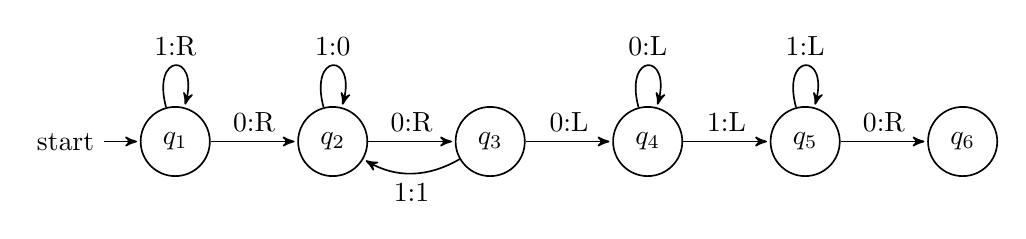
\begin{tikzpicture}[->,>=stealth',shorten >=1pt,auto,node distance=2cm,semithick]
		\tikzstyle{every state}=[circle]
		
		\node[initial,state] (A)		{$q_1$};
		\node[state] (B) [right of=A] 	{$q_2$};
		\node[state] (C) [right of=B]	{$q_3$};
		\node[state] (D) [right of=C]	{$q_4$};
		\node[state] (E) [right of=D]	{$q_5$};
		\node[state] (F) [right of=E]	{$q_6$};
		
		\path (A) edge [loop above]	node {1:R} (A)
			       edge 				node {0:R} (B)
			 (B) edge [loop above]	node {1:0}  (A)
			       edge				node {0:R} (C)
			 (C) edge [bend left]		node {1:1} (B)
			       edge				node {0:L} (D)
			 (D) edge [loop above]	node {0:L} (D)
			       edge				node {1:L} (E)
			 (E) edge [loop above]	node {1:L} (E)
			       edge				node {0:R} (F);

	\end{tikzpicture}
	
\bigskip
	
	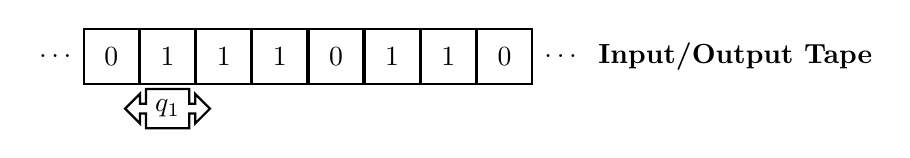
\begin{tikzpicture} [start chain=1 going right, node distance=-0.15mm]
		    \tikzstyle{every path}=[thick]
		    \tikzstyle{tmtape}=[draw,minimum size=\sizetape]
		    \tikzstyle{tmhead}=[arrow box,draw,minimum size=.5cm,arrow box
		    arrows={east:.25cm, west:0.25cm}]
		    \edef\sizetape{0.7cm}
		    \node [on chain=1,tmtape,draw=none] {$\ldots$};
		    \node [on chain=1,tmtape] {0};
		    \node [on chain=1,tmtape] (input) {1};
		    \node [on chain=1,tmtape] {1};
		    \node [on chain=1,tmtape] {1};
		    \node [on chain=1,tmtape] {0};
		    \node [on chain=1,tmtape] {1};
		    \node [on chain=1,tmtape] {1};
		    \node [on chain=1,tmtape] {0};
		    \node [on chain=1,tmtape,draw=none] {$\ldots$};
		    \node [on chain=1] {\textbf{Input/Output Tape}};
		    \node [tmhead,yshift=-.3cm] at (input.south) (head) {$q_1$};
	\end{tikzpicture}
	
\bigskip

\subsection*{Translation into first order logic:}

\bigskip

Our representation will take the form $\Delta \models H$, where $\Delta$ is a set of statements in 
first order logic and $H$ is a single statement logically entailed from $\Delta$. Our language has 
the domain $\mathbb{Z}$ of negative integers, 0 and positive integers. Special features of the language
referred to in the following logical statements include the successor function $(')$, the constant \textbf{0}
(which denotes the integer 0), the two-place ordering predicate $<$, the two-place state predicate \textbf{Q}, 
and the two-place "scanning" predicate \textbf{S}.
\\\\
We first have to encode some mathematical facts about $'$ and $<$ :

\begin{equation}
\forall z \exists x \: z=x' \land \forall z \forall x \forall y ([z=x' \land z=y'] \rightarrow x = y) 
\end{equation}	
\\\\
and:
\begin{multline}
\forall x \forall y \forall z [(x<y \land y<z) \rightarrow x<z] \; \land \; \forall x \forall y (x'=y \rightarrow x<y) 
\; \\ \land \; \forall x \forall y (x<y \rightarrow x \neq y).
\end{multline}
\\\\
Next we need to encode the initial configuration of the tape:


\begin{multline}
\textbf{0} Q_{1} \textbf{0} \land \textbf{0} S_{1} \textbf{0} \land \textbf{0} S_{1} \textbf{0}' \land
\textbf{0} S_{1} \textbf{0}'' \land \textbf{0} S_{1} \textbf{0}'''' \land \textbf{0} S_{1} \textbf{0}''''' \land \\
\forall y [(y \neq \textbf{0} \land y \neq \textbf{0}' \land y \neq \textbf{0}'' \land y \neq \textbf{0}'''' 
\land y \neq \textbf{0}''''') \rightarrow \textbf{0}S_{0}y]
\end{multline}
\\\\
To finish $\Delta$ we encode each of the state transitions (arrows in the flow graph) as logical statements:

\begin{equation}
\forall t \forall x [(tQ_{1}x \land tS_{1}x) \rightarrow (t'Q_{1}x' \land \forall y [(tS_{0}y \rightarrow t'S_{0}y) 
\land (tS_{1}y \rightarrow t'S_{1}y)])]
\end{equation}

\begin{equation}
\forall t \forall x [(tQ_{1}x \land tS_{0}x) \rightarrow (t'Q_{2}x' \land \forall y [(tS_{0}y \rightarrow t'S_{0}y)
\land (tS_{1}y \rightarrow t'S_{1}y)])]
\end{equation}

\begin{multline}
\forall t \forall x [(tQ_{2}x \land tS_{1}x) \rightarrow \\ ([t'Q_{2}x \land t'S_{0}x] \land \forall y [(y \neq x) 
\rightarrow ([tS_{0}y \rightarrow t'S_{0}y] \land [tS_{1}y \rightarrow t'S_{1}y])])]
\end{multline}

\begin{equation}
\forall t \forall x [(tQ_{2}x \land tS_{0}x) \rightarrow (t'Q_{3}x' \land \forall y [(tS_{0}y \rightarrow t'S_{0}y)
\land (tS_{1}y \rightarrow t'S_{1}y)])]
\end{equation}

\begin{equation}
\forall t \forall x [(tQ_{3}x' \land tS_{0}x') \rightarrow (t'Q_{4}x \land \forall y [(tS_{0}y \rightarrow t'S_{0}y)
\land (tS_{1}y \rightarrow t'S_{1}y)])]
\end{equation}

\begin{multline}
\forall t \forall x [(tQ_{3}x \land tS_{1}x) \rightarrow \\ ([t'Q_{2}x \land t'S_{1}x] \land \forall y [(y \neq x)
\rightarrow ([tS_{0}y \rightarrow t'S_{0}y] \land [tS_{1}y \rightarrow t'S_{1}y])])]
\end{multline}

\begin{equation}
\forall t \forall x [(tQ_{4}x' \land tS_{0}x') \rightarrow (t'Q_{4}x \land \forall y [(tS_{0}y \rightarrow t'S_{0}y)
\land (tS_{1}y \rightarrow t'S_{1}y)])]
\end{equation}

\begin{equation}
\forall t \forall x [(tQ_{4}x' \land tS_{1}x') \rightarrow (t'Q_{5}x \land \forall y [(tS_{0}y \rightarrow t'S_{0}y)
\land (tS_{1}y \rightarrow t'S_{1}y)])]
\end{equation}

\begin{equation}
\forall t \forall x [(tQ_{5}x' \land tS_{1}x') \rightarrow (t'Q_{5}x \land \forall y [(tS_{0}y \rightarrow t'S_{0}y)
\land (tS_{1}y \rightarrow t'S_{1}y)])]
\end{equation}

\begin{equation}
\forall t \forall x [(tQ_{5}x \land tS_{0}x) \rightarrow (t'Q_{6}x' \land \forall y [(tS_{0}y \rightarrow t'S_{0}y) 
\land (tS_{1}y \rightarrow t'S_{1}y)])]
\end{equation}
\\\\
The last statement to encode is $H$, which is the disjunction of all sentences stating the machine is in a 
potential halting state:

\begin{multline}
\\ \exists t \exists x (tQ_{1}x \land tS_{0}x) \lor \exists t \exists x (tQ_{1}x \land tS_{1}x) \lor \\
\exists t \exists x (tQ_{2}x \land tS_{0}x) \lor \exists t \exists x (tQ_{2}x \land tS_{1}x) \lor \\
\exists t \exists x (tQ_{3}x \land tS_{0}x) \lor \exists t \exists x (tQ_{3}x \land tS_{1}x) \lor \\
\exists t \exists x (tQ_{4}x \land tS_{0}x) \lor \exists t \exists x (tQ_{4}x \land tS_{1}x) \lor \\
\exists t \exists x (tQ_{5}x \land tS_{0}x) \lor \exists t \exists x (tQ_{5}x \land tS_{1}x) \lor \\
\exists t \exists x (tQ_{6}x \land tS_{0}x) \lor \exists t \exists x (tQ_{6}x \land tS_{1}x) \lor \\
\end{multline}

(is halting symbol separate from blank and mark?)
\end{document}